\section{Frontend Electronics}

This chapter serves as a technical documentation of the electronics currently in use and under development for MTT.

\subsection{APDPI}

The Avalanche Photodiode Power Interface (APDPI) is a standard NIM module that supplies power for the SiPMs, amplifier circuits and logic of the frontend electronics.
Figure \ref{APDPI_front} shows the front panel of an APDPI module: On the top there is a DSUB-9 connector consisting of a VBIAS, V+, V-, GND, RTX+ and RTX- output.
Below the connector there are two switches BIAS and POWER and again below that a USB B plug.

The $+12\,\text{V}$ line of the NIM backend is fed to a DC-DC converter that is adjustable via a potentiometer located next to the converter.
The converter takes $10.8\,\text{V} .. 13.2\,\text{V}$ and outputs $0\,\text{V} .. 180\,\text{V}@15\,\text{mA}$ to the VBIAS line. The BIAS switch is located directly below the
DSUB-9 connector and switches VBIAS on and off. The typical VBIAS voltage currently used is $82\,\text{V}$.

V+ and V- supply a $\pm3.3\,\text{V}@1\text{A}$ power source respectively for the amplifier and logic circuits of the frontend electronics. There are two voltage regulators 
which use the $\pm6\,\text{V}$ lines of the NIM backend to generate the $\pm3.3\,\text{V}$ outputs. Below the VBIAS switch there is also a POWER switch located for V+ and V-.

GND is the reference potential for VBIAS as well as for V+ and V-. It uses the ground line of the NIM backend and is also connected to the casing of the 
module to reduce noise.

RTX+ and RTX- are the differential EIA-485 compliant outputs used for communication with and slow control of the frontend electronics. The EIA-485 (or RS-485) 
defines a physical layer that uses a differential signal for communcation thus providing a stable signal over distances of up to $1.2\,\text{km}$. The data link layer is 
compliant to the microcontroller friendly Universal Synchronous/Asynchronous Receiver Transmitter (USART) which simplifies the whole commucation chain in hardware. 
A computer can be connected to the APDPI via a USB B plug located beneath the POWER switch. The USB signal is mapped to USART by a \emph{FT232RL} 
chip and again converted to RS-485 by a \emph{MAX3086E} chip thus the slow control can be accessed with a simple 
FTDI serial driver.
The \emph{MAX3086E} transceiver provides a half duplex communication interface meaning that the driver uses the same data lines to transmit and receive data.

	\begin{figure}[t]
		\centering
			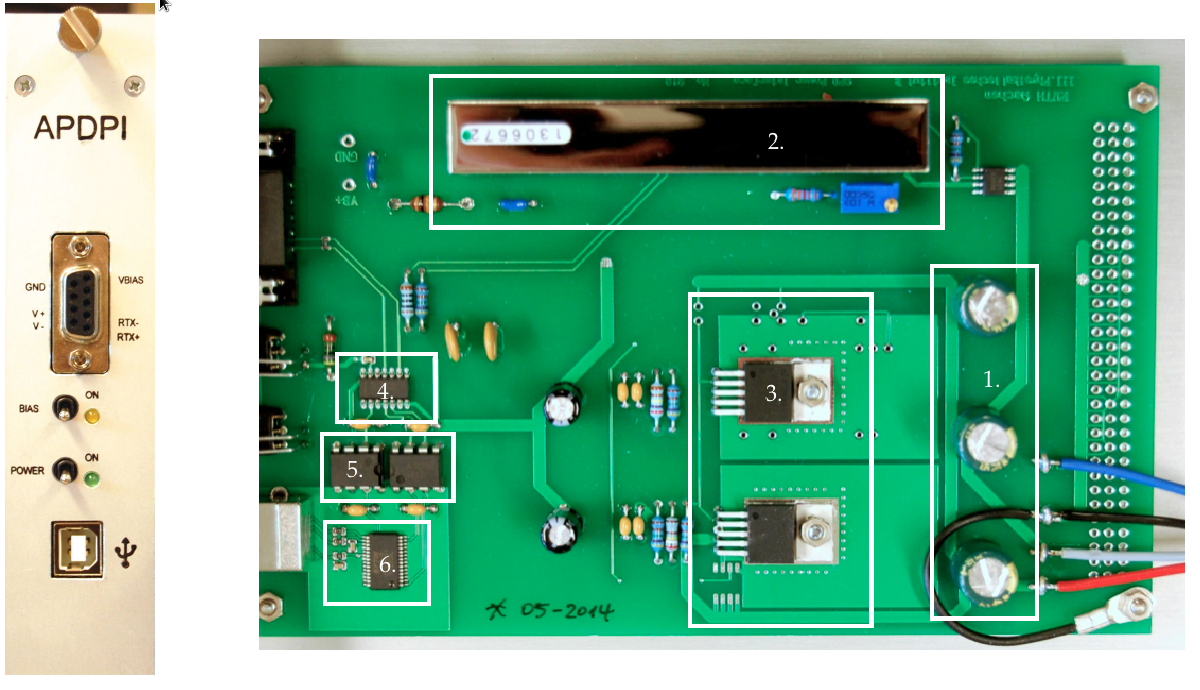
\includegraphics[width=1.0\textwidth]{Figures/weinstock/apdpi.png}
		\caption{\textbf{Left:} Front plate of an APDPI. \textbf{Right:} APDPI circuit: 1. $470\,\mu \text{F}$ bypass capacitors for the $\pm6\,\text{V}$ and $12\,\text{V}$ 
												   NIM lines;
												2. DC-DC converter and regulation potentiometer;
												3. $\pm3.3\,\text{V}$ voltage regulators with heat sink area;
												4. MAX3086E RS-485 to UART converter.
												5. Opto-isolators for electrical isolation of the FT232RL circuit. This circuit runs
												at $5\,\text{V}$ provided by the USB host;
												6. FT232RL UART to USB converter.}
		\label{APDPI_front}
	\end{figure}	

\subsubsection{SiPM Bus}

The SiPM Bus defines the application layer for the serial communication with the frontend electronics. The bus is host driven, so the bus master has to query for data from the slaves.
To ensure the correct understanding of the sent commands each individual byte is echoed by the slave and should be checked. To start the communication the bus master sends the start
delimiter character '$<$' (ASCII \verb|0x3C|) and claims the bus (start delimiter will not be echoed). Any further try to claim the bus will fail because the bus is now busy. 
The start delimiter then is followed by a unique 8 bit slave address which is echoed by the slave. The slave is now addressed and is ready to receive commands. For a complete list of
implemented commands and a short description see table \ref{sipm_bus_table}. Every command and parameter needed by the command will be echoed bytewise aswell. In addition to the echo 
the slave will send the End Of Message (EOM) string "\textbackslash n \textbackslash r *" (ASCII \verb|0x0A|, \verb|0x0D|, \verb|0x2A|) after receiving a complete command line including all parameters. Once all commands have been issued to the frontend electronics the communication is terminated by sending the stop delimiter '$>$' (ASCII \verb|0x3E|) and the bus is freed. 

Currently the transmission rate is limited to 9600 BAUD to reduce power consumption of the microcontroller on the frontend electronics and the framing is set to 8N1 meaning eight 
bits of data per frame, no parity bit, one stop bit to maximize data throughput.

	\begin{table}
		\begin{center}
			\begin{tabular}[]{|l||p{6cm}|p{4cm}|}
			\hline
			Command & Description & Example \\
			\hline
			"A" or "B" & Read temperature adjusted bias voltage of SiPM A or B. Ranges from $0x0000..0x3FFF$ in counts of $5\,\text{mV}$. & Send: "A"
			\newline Receive: "A1234\textbackslash r\textbackslash n*"\\
			\hline
			"D" or "E" & Set bias voltage at $25\,^{\circ} \text{C}$ for SiPM A or B. Ranges from $0x0000..0x3FFF$ in counts of $5\,\text{mV}$. Changes are only 
			temporary and will be lost after reset.& Send: "D1234"\newline Receive: "D1234\textbackslash r\textbackslash n*"\\
			\hline
			"I" & Read temperature in $^{\circ}\text{C}$. & Send: "I" \newline Receive: "I23.567\textbackslash r\textbackslash n*" \\
			\hline
			"J" & Read raw temperature in ADC counts. Ranges from $0x000..0x3FF$. & Send: "J" \newline Receive: "J234\textbackslash r\textbackslash n*" \\
			\hline
			"C" & Read temperature coefficient. Ranges from $0x00..0x7F$ in counts of $1\,\frac{\text{mV}}{\text{K}}$. & Send: "C" 
			\newline Receive: "C39\textbackslash r\textbackslash n*" \\
			\hline
			"F" & Set temperature coefficient. Ranges from $0x00..0x7F$ in counts of $1\,\frac{\text{mV}}{\text{K}}$. Changes are only temporary and 
			will be lost after reset. & Send: "F10" \newline Receive: "F10\textbackslash r\textbackslash n*" \\
			\hline
			"H" & Prints hard- and firmware version of the module. & Send: "H" \newline Receive: "HHW Version 2.1 SW Version 2.0\textbackslash r\textbackslash n*" \\
			\hline
			"S" & Prints serial number and default bias at $25\,^{\circ} \text{C}$ in counts of $5\, \text{mV}$ of all SiPMs on the module. &  Send: "S" 
			\newline Receive: "S Sensor A No.: 3H000004 Voltage:3567 Sensor B No.: 3H000005 Voltage:3565\textbackslash r\textbackslash n*" \\
			\hline
			"Q" & Switch module to DAC calibration mode. & Send: "Q" \newline Receive: "Q\textbackslash r\textbackslash n*" \\
			\hline
			\end{tabular}
		\end{center}
		\caption{Overview of all commands supported by firmware version $<2.0$. Note that modules with only one SiPM neither support command "B" nor "E".}
		\label{sipm_bus_table}
	\end{table}

\subsection{MPPC Dou Controller}

The Multi Pixel Photon Counter Duo Controller (MPPC\_D) is the current frontend electronics prototype for the MTT project. It features regulated bias voltages for up to two SiPMs, 
a Pt100 based temperature probe, one LEMO output for each single SiPM and a sum channel LEMO output.

The core part of the MPPC\_D is an \emph{ATmega88P}. The \emph{ATmega88P} is an 8 bit microcontroller designed for very low power consumption, features a 
USART interface, 10 bit DACs, a Serial Peripheral Interface (SPI), $512\,B$ of EEPROM and runs at $1\,\text{MHz}$ system clock to minimize power consumption. 

The MPPC\_D can be connected to the APDPI by a ribbon cable featuring a male DSUB-9 connector and one or several 6 pin jacks which can be plugged into the boxed 6 pin header
located on the frontend board. When connecting multiple MPPC\_Ds to one APDPI one must not only consider address conflicts, but also power consumption of the modules for the APDPI
can supply only $15\,\text{mA}@82\,\text{V}$ and $1\,\text{A}@\pm3.3\,\text{V}$. The RTX+ and RTX- lines from the APDPI are directly fed into a \emph{MAX13430E} low power RS-485 
transceiver chip and is used by the microcontroller's USART for serial communication using the SiPM bus protocol.  
Figure \ref{mppc_top} shows a picture of all functional units of the frontend board.
	
	\begin{figure}[t]
		\centering
			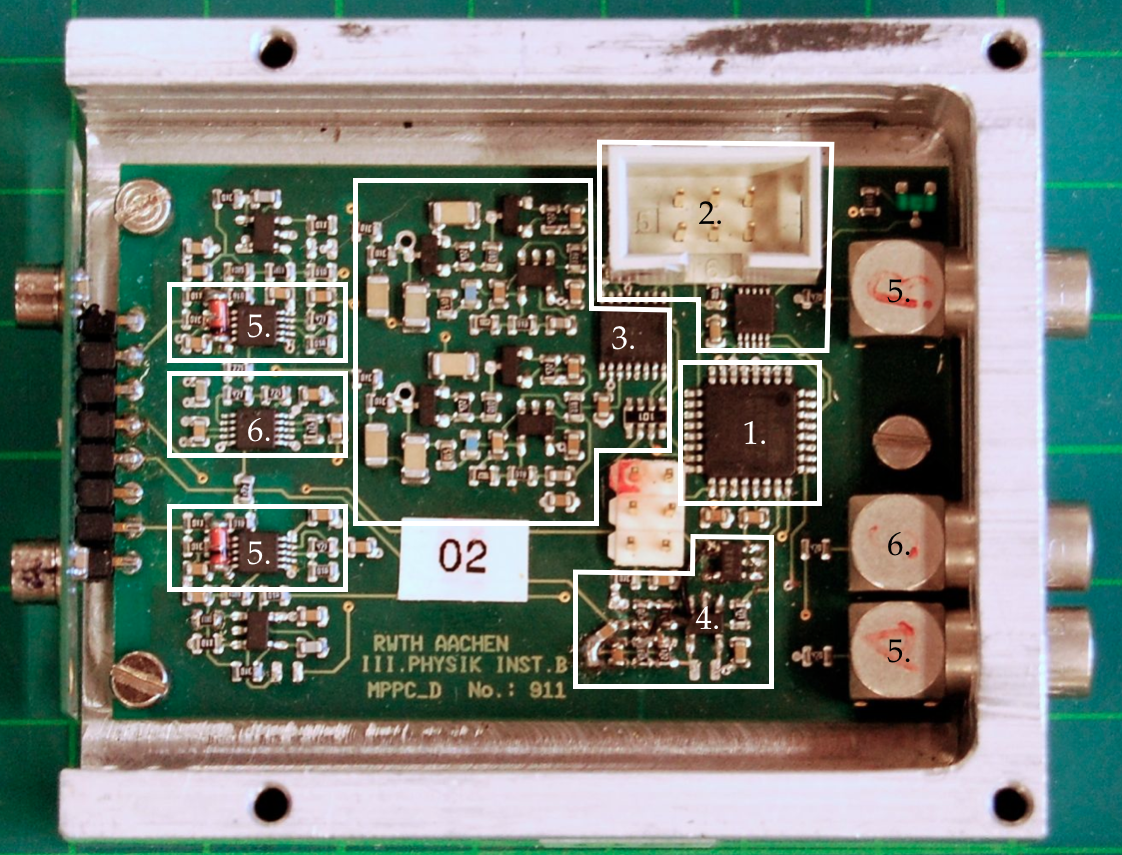
\includegraphics[width=0.5\textwidth]{Figures/weinstock/mppc_d_titled.png}
		\caption{Top down view of the MPPC\_Ds circuitry: 1. ATmega88P with it's 6 pin ICSP header on the bottom left; 
								  2. Boxed 6 pin header for SiPM bus connector;
								  3. Two voltage regulators $0..82\,\text{V}$ (VBIAS) for the SiPMs;
								  4. Pt100 based temperature probe. The Pt100 resistor is located on the front plate between both SiPMs. 
								       It's analog signal is passed to this circuitry;
								  5. Preamplifier and shaper stages and corresponding LEMO outputs; 
								  6. Summing amplifier and LEMO output;
			}
		\label{mppc_top}
	\end{figure}	

\newpage

\subsubsection{Temperature Measurement}

Because of the strong temperature dependency of the SiPMs output pulses a precise temperature measurement is needed to adjust the bias voltage of the SiPMs. The temperature probe of
the MPPC\_D calculates the temperature by measuring the resistance of a Pt100 resistor. The probe's circuit consists of a Wheatstone bridge including the Pt100, an amplifier circuit using
the \emph{MAX4040} OpAmp to compensate the non linearities of the bridge and another MAX4040 OpAmp as a buffer to supply the probe with the
internal Analog Reference (AREF) of $1.1\,\text{V}$ from the microcontroller as shown in Figure \ref{pt100_probe}.

The resistance of the Pt100 changes as follows:
	\begin{equation}
		R_{Pt100}(T) = R_0(1 +\alpha_T T + \beta_T T^2 + \mathcal{O}(T^3)),
		\label{eq_pt100_temperature}
	\end{equation}
where $R_0 = R_{Pt100}(0^{\circ} \text{C})=100\,\Omega$, $\alpha_T = 3.9083 \times 10^{-3}\, \text{K}^{-1}$ and $\beta_T = -5.775 \times 10^{-7}\, \text{K}^{-2}$. To compensate 
the non linear terms in equation \ref{eq_pt100_temperature}, which are lowering the resistance at higher temperatures, current can be fed back to the Pt100 resistor to increase 
the output voltage. The current feedback should be chosen in a manner that the resulting output voltage of the temperature probe changes linear with respect to the temperature.

One also has take into account the non linearities resulting from the Wheatstone bridge. The output voltage $U_{in}$ that is fed into the MAX4040 amplifier is
	\begin{equation}
		U_{in} = U_{ref}(\frac{R_{10}}{R_{10} + R_5} - \frac{R_{11}}{R_{11} + R_6}).
	\end{equation}
As shown in the schematics in Figure \ref{pt100_probe} $R_{10}$ is the Pt100 resistor. One can easily see that the output voltage is not linear dependent on the resistance
of $R_{10}$. To reduce the effect of this non linearity $R_{5}$ is chosen to be larger than $R_{10}$, so that $R_{10} + R_{5} \approx R_{5}$ holds. The resistors $R_6$, $R_9$ and 
$R_{11}$ set the required gain and offset of the amplifier to produce the desired output voltage. 
$R_7$ provides the previously discussed current feedback to the Pt100 resistor depending on the output of the amplifier.

	\begin{figure}[t]
		\centering
			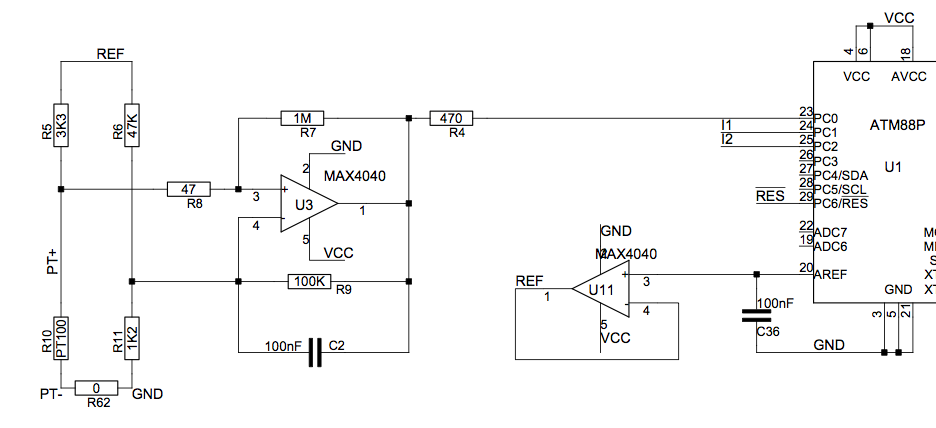
\includegraphics[width=0.7\textwidth]{Figures/weinstock/pt100_probe.png}
		\caption{Schematics of the Pt100 based temperature probe of the MPPC\_D. The resistor $R_{10}$ is the Pt100 resistor.}
		\label{pt100_probe}
	\end{figure}	
 
\subsubsection{Temperature Probe Calibration}

The output voltage of the temperature probe is measured by a $10$ bit ADC on the microcontroller. Internally the temperature then is calculated by the following equation:
\begin{equation}
	T[^{\circ}C] = TGain[^{\circ}C/count] \times ADCcount + TOffset[^{\circ}C]
\end{equation}
The calibration of the temperature probe can be done by simply exposing the probe to a well regulated temperature and reading it's ADC register. The $10$ bit ADC of the microcontroller
can be read out with the command "J". For a fast temperature calibration one also can use a Pt100 simulator. This simulator is a potentiometer that can be set to a certain 
temperature value and outputs the corresponding resistance of a Pt100 resistor at the given temperature value. 

\newpage

\subsubsection{Bias Voltage Supply}

To compensate the temperature effects on the SiPM the bias voltage has to be corrected by a factor of $\frac{\Delta U_{bias}}{\Delta T} = 56\,\frac{mV}{K}$. The MPPC\_D has two 
voltage regulators to apply the correct bias voltage to each SiPM. The schematics of a voltage regulator are shown in Figure \ref{voltage_regulator}. 
	
	\begin{figure}[t]
		\centering
			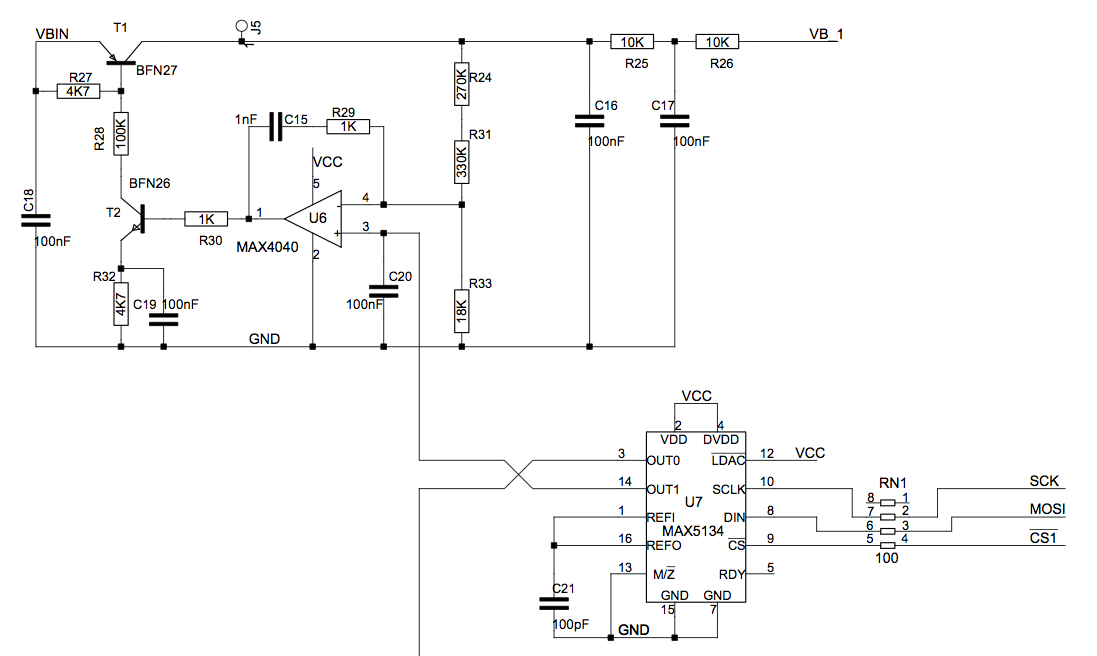
\includegraphics[width=0.7\textwidth]{Figures/weinstock/dac_circuit.png}
		\caption{Schematics of one of the voltage regulators on the MPPC\_D. The regulated bias voltage is output to $VB_1$.}
		\label{voltage_regulator}
	\end{figure}	

The voltage regulators use a Pulse Width Modulation (PWM) signal to adjust the bias voltages. PWM is used to reduce power consumption.
The core parts of the voltage regulator are two high voltage transistors $T_1$ and $T_2$ and an integrating amplifier circuit built around another MAX4040. The integrator increases
it's output voltage as long as the voltage drop at the divider $R_{24}$, $R_{31}$ and $R_{33}$ is below the voltage input of the 16 bit MAX5134 DAC.
The voltage on the voltage divider is increased by the output of $T_1$ which again is influenced by the amplifier's output. The result of this feedback is a rectangular output
pulse at $T_1$. The duty cycle of this pulse is determined by ratio of the voltage given by the DAC and the voltage drop of the divider:
	\begin{eqnarray}
		D &=& \frac{T}{P} = \frac{U_{dac}}{U_{div}} \\
		U_{div} &=& \frac{R_{33}}{R_{24} + R_{31} + R_{33}} U_{bin} = 2.46\,\text{V},
	\end{eqnarray}
where $T$ is the time the signal is active, $P$ the total period of the signal ($P$ is determined by the values of $C_{22}$ and $R_{29}$) and $U_{bin}=82V$ the voltage provided by the 
APDPIs VBIAS line. The output voltage of the DAC ranges from $U_{dac}=0\, \text{V} .. 2.44\, \text{V}$ (internal reference). The PWM output is then filtered by the two high passes 
$R_{25}$, $C_{16}$ and $R_{26}$, $C_{17}$ ($f_{crit} = \frac{1}{2 \pi RC}$) and transferred to the SiPM. The applied bias voltage is then defined by the duty cycle of the former 
PWM signal:
	\begin{equation}
		U_{bias} = U_{bin} D = U_{bin} \frac{U_{dac}}{U_{div}}.
	\end{equation}

\subsubsection{Bias Voltage Regulator Calibration}
The output voltage of the DAC is set by accessing the output registers. The output registers can be set to any value between \verb|0x0000| .. \verb|0xFFFF|, setting the output to 
$0\, \text{V}..2.44\, \text{V}$ respectively. To get the precise conversion from DAC counts to output bias voltage one must perform a calibration of the DACs. Internally 
the bias voltage set by the following calculation:
	\begin{eqnarray}
		DACcounts &=& DACOffset + U_{adj}[5\,mV]/DACGain \\
		U_{adj} &=& \frac{\Delta U_{bias}}{\Delta T}(T - 25\,^{\circ} \text{C}) + U_{adj}(25\,^{\circ} \text{C}),
	\end{eqnarray} 
where $U_{adj}$ is the temperature adjusted bias voltage and $\frac{\Delta U_{bias}}{\Delta T} = 56\,\frac{\text{mV}}{\text{K}}$. 

To calibrate the DAC the module has to be set to DAC calibration mode by issuing the command "Q". In calibration mode $DACOffset$ and $\frac{\Delta U}{\Delta T}$ 
are set to $0$ and $DACGain$ to $1$ thus disabling the temperature correction. Also one can now access the DACs registers directly by setting the bias voltage 
at $25^{\circ} \text{C}$ with the command "Dhhhh" or "Ehhhh" to the hex value $5\times\verb|0xhhhh|$. By setting the DAC output registers to a given value and then measuring the 
output adjusted bias voltage one can easily perform a calibration.

\subsubsection{Amplifier Circuits}

The MPPC\_D uses Current Feedback Amplifiers (CFA) instead of Voltage Feedback Amplifiers (VFA) because of the superior gain-bandwidth product of these amplifiers. A high 
gain-bandwidth product is needed because the Geiger discharges on the SiPM create high speed rising edges. The steep rising edges provide the fastest information of an incoming photon. 
By not distorting these high speed components the trigger information becomes avaliable faster.

The amplifier chip used on the MPPC\_D is the \emph{MAX4228} which has a bandwidth of $1\,\text{GHz}$ at unity gain. The whole amplifier circuit is shown in Figure \ref{fig:amp_cir}. 
The first amplification stage is a transimpedance amplifier. This preamplifier converts a current signal into a voltage signal:
\begin{equation}
	U_{preamp} = R_{20} I_{sig},
\end{equation}
where $R_{20} = 1\,\text{k}\Omega$. The second stage is a non-inverting amplifier, but only half the preamplifier's signal reach this step for the other half is fed to the summing amplifier:
\begin{equation}
	U_{out} = \frac{1}{2} (1 + \frac{R_{23}}{R_{22}}) \, U_{preamp} = 2.85 \, U_{preamp}.
\end{equation}

	\begin{figure}[t]
		\centering
			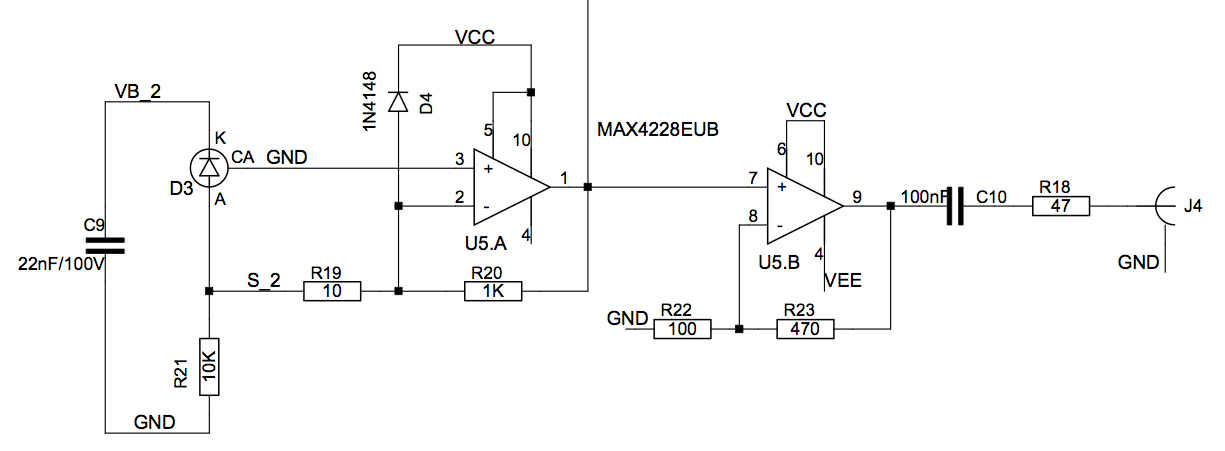
\includegraphics[width=0.7\textwidth]{Figures/weinstock/amplifier_circuit.png}
		\caption{Schematics of one of the amplifier circuits. The first stage is the tansimpedance preamplifier, the second is a non-inverting amplifier. The capacitor is used to decouple the AC from the DC components since we are only interested in the AC components of the pulse.}
		\label{fig:amp_cir}
	\end{figure}	
The summing amplifier shown in Figure \ref{fig:sum_amp} adds the signals of both preamplifiers and amplifies them again by a factor of $\approx4.5$. So in total the sum signal is about $80\%$ smaller than the single channel signal.

	\begin{figure}[t]
		\centering
			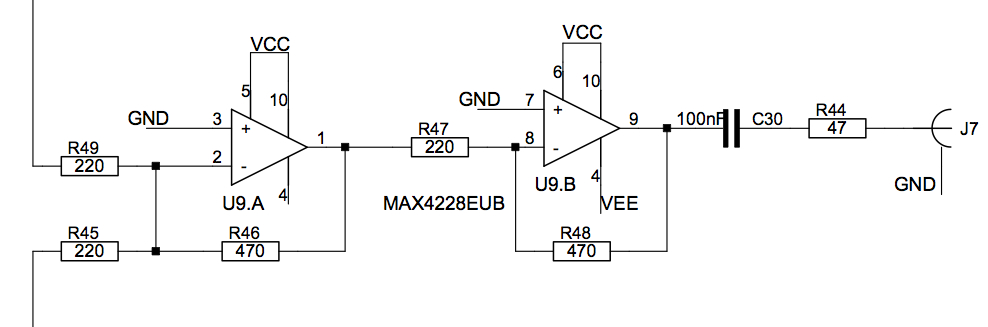
\includegraphics[width=0.7\textwidth]{Figures/weinstock/sum_amp.png}
		\caption{Summing amplifier of the MPPC\_D. The inputs of the first amplifying stage come directly from preamplifiers.}
		\label{fig:sum_amp}
	\end{figure}	

	
One of the drawbacks of CFAs is that they have a high offset current which results in a offset voltage of about $U_{off,CFA}\approx \pm 1\,\text{V}$. Because we are only interested in the AC components of the signal we use $C_{10}$ as a decoupling capacitor. The resistor $R_{18}$ adjusts the lines impedance to the resistance of a LEMO cable to reduce current reflections.

Figure \ref{fig:sipm_pulse_old} shows a 1 P.E. output from the amplifier stages. The pulse height is about $U_{1p.e.} = 25\,\text{mV}$ and the total pulse duration $T_{pulse} = 80\,\text{ns}$. Figure \ref{fig:rise_time_old} shows a rise time distribution for $10,000$ SiPM pulses. As one can see the rise time of an average SiPM pulse is at about $t_{rise} = 5\,\text{ns}$.

	\begin{figure}[t]
		\centering
			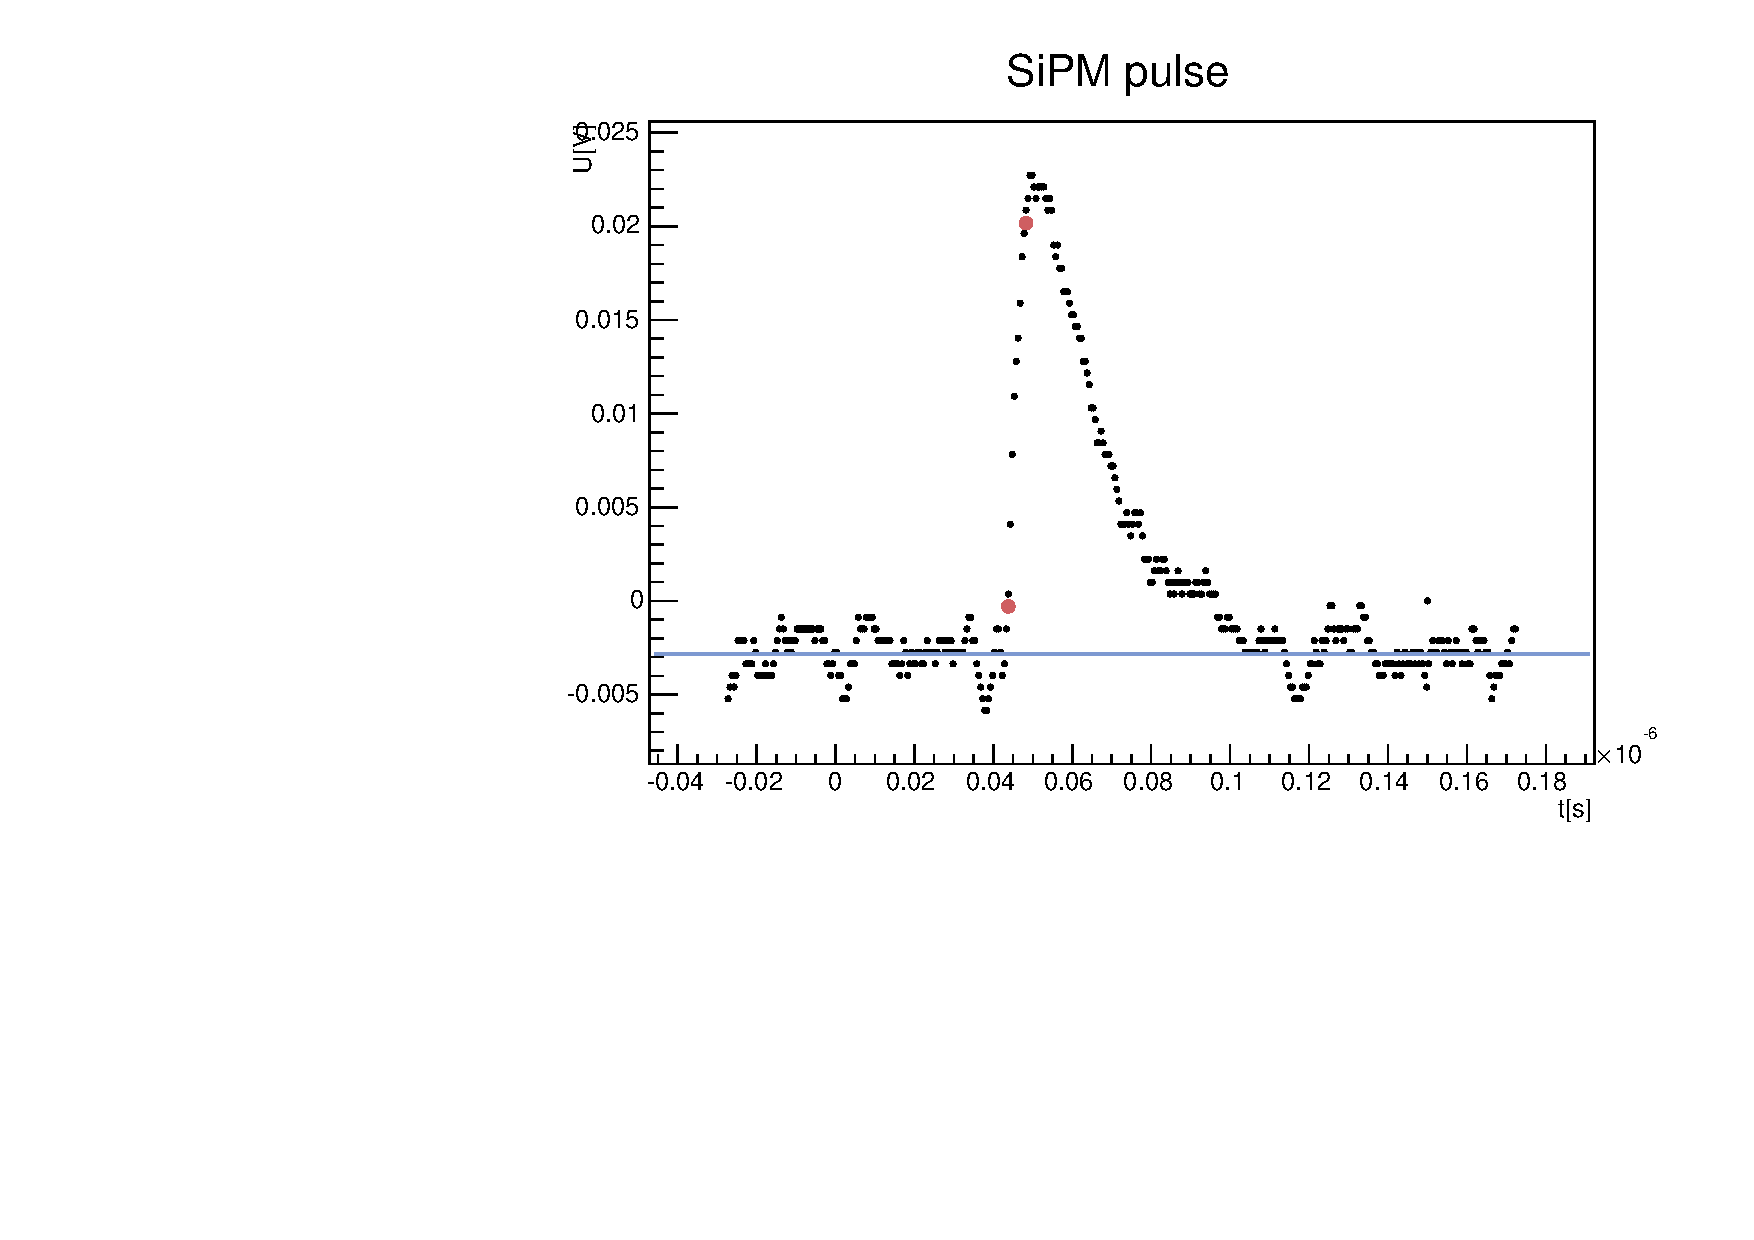
\includegraphics[width=0.7\textwidth]{Figures/weinstock/old_amp_1pe.pdf}
		\caption{1 P.E. output pulse of the SiPM after amplification by the MPPC\_D. The blue line is the reconstructed baseline, the red dots are the $10\%$ and $90 \%$ marks of the pulse height. They are used to calculate the rise time.}
		\label{fig:sipm_pulse_old}
	\end{figure}
	
	\begin{figure}[t]
		\centering
			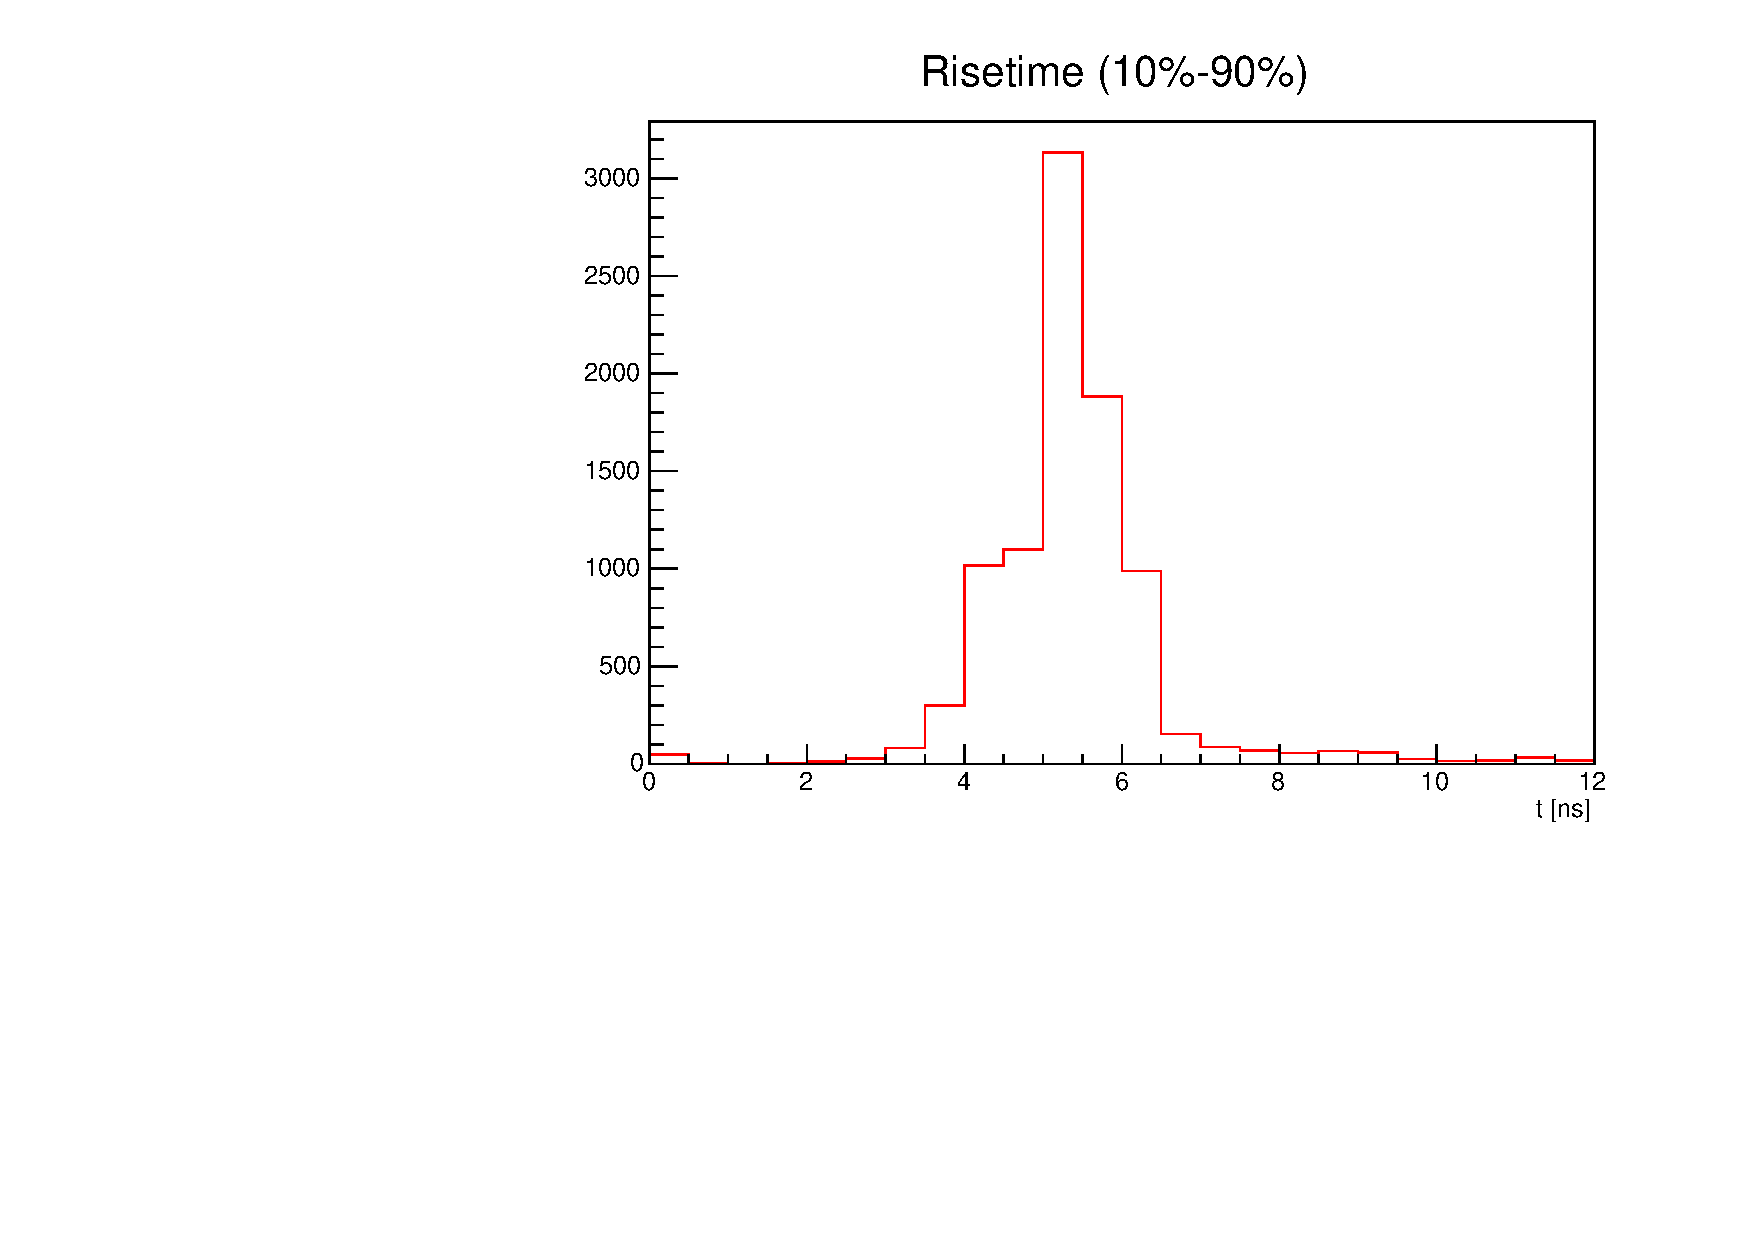
\includegraphics[width=0.7\textwidth]{Figures/weinstock/old_amp_rise_time.pdf}
		\caption{Distribution of rise times of $10,000$ SiPM pulses amplified by the MPPC\_D amplifier stages.}
		\label{fig:rise_time_old}
	\end{figure}	

\subsubsection{Overview Of Technical Characteristics}

\subsection{Appendix: Circuit Diagrams}
